\documentclass[a4paper,12pt]{article}

\usepackage[T2A]{fontenc}			
\usepackage[utf8]{inputenc}			
\usepackage[english,russian]{babel}	

\usepackage[
bookmarks=true, colorlinks=true, unicode=true,
urlcolor=black,linkcolor=black, anchorcolor=black,
citecolor=black, menucolor=black, filecolor=black,
]{hyperref}

\usepackage{color}
\usepackage{caption}
\DeclareCaptionFont{white}{\color{black}}
\DeclareCaptionFormat{listing}{\colorbox{white}{\parbox{\textwidth}{#1#2#3}}}
\captionsetup[lstlisting]{format=listing,labelfont=white,textfont=white}

\usepackage{amsmath,amsfonts,amssymb,amsthm,mathtools} 
\usepackage{wasysym}

\usepackage{graphicx}
%\usepackage[cache=false]{minted}
\usepackage{cmap}
\usepackage{indentfirst}

\usepackage{listings} 
\usepackage{fancyvrb}

\usepackage{geometry}
\geometry{left=2cm}
\geometry{right=1.5cm}
\geometry{top=1cm}
\geometry{bottom=2cm}

\setlength{\parindent}{5ex}
\setlength{\parskip}{0.5em}

\usepackage{pgfplots}

\usepackage{longtable}

\begin{document}
	\lstset{ %
		language=C,                 % выбор языка для подсветки (здесь это С)
		basicstyle=\small\sffamily, % размер и начертание шрифта для подсветки кода
		numbers=left,               % где поставить нумерацию строк (слева\справа)
		numberstyle=\tiny,           % размер шрифта для номеров строк
		stepnumber=1,                   % размер шага между двумя номерами строк
		numbersep=5pt,                % как далеко отстоят номера строк от подсвечиваемого кода
		backgroundcolor=\color{white}, % цвет фона подсветки - используем \usepackage{color}
		showspaces=false,            % показывать или нет пробелы специальными отступами
		showstringspaces=false,      % показывать или нет пробелы в строках
		showtabs=false,             % показывать или нет табуляцию в строках
		frame=single,              % рисовать рамку вокруг кода
		tabsize=2,                 % размер табуляции по умолчанию равен 2 пробелам
		captionpos=t,              % позиция заголовка вверху [t] или внизу [b] 
		breaklines=true,           % автоматически переносить строки (да\нет)
		breakatwhitespace=false, % переносить строки только если есть пробел
		escapeinside={\%*}{*)}   % если нужно добавить комментарии в коде
	}
	
	% Титульный лист
	\begin{figure}[h!]
		\begin{center}
			{
\includegraphics[scale = 0.4]{titul.jpg}}
			\label{titul}
		\end{center}
	\end{figure}
	
	\vspace*{15mm} 
	
	\huge
	\begin{center}
		Дисциплина: <<Моделирование>>
	\end{center}
	
	\begin{center}
		Лабораторная работа №3
	\end{center}

	
	\huge
	\begin{center}
		Тема работы:\\
		<<Марковские случайные цепи>>
	\end{center}
	\vspace*{25mm} 
	
	\large
	\begin{flushright}
		Студент: Левушкин И. К. \\
		Группа: ИУ7-72Б \\
		Преподаватель: Рудаков И. В. \\
	\end{flushright}
	
	\vspace*{25mm}
	\begin{center}
		Москва, 2020 г.  
	\end{center}
	\thispagestyle{empty}
	
	
	\newpage
	
	\section*{Задание}
	
	Необходимо для сложной системы $S$, имеющей не более 10 состояний, определить среднее время нахождения системы в предельных состояниях, т. е. при установившемся режиме работы. Матрица интенсивностей, задать размерность системы ($\leqslant 10$), нажать на кнопку вычислить и получить время.
	
	\section*{Марковский случайный процесс}
	
	Случайный процесс называется марковским, если он обладает следующим свойством: для каждого момента времени $t_0$ вероятность любого состояния системы в будущем зависит только от её состояния в настоящем, т. е. при $t = t_0$, и не зависит от того, когда и каким образом система пришла в это состояние, т. е. не зависит от того, как процесс развивался в прошлом. В марковском случайном процессе будущее развитие его зависит только от настоящего и не зависит от предыстории процесса. Уравнения Колмогорова:
	
	\begin{equation}
	F = (P'(t), P(t), \Lambda) = 0,
	\end{equation}
	
	$\Lambda = \lambda_1, \lambda_2, ..., \lambda_n$ - набор некоторых коэффициентов.
	
	
	Для станционарного распределения:
	
	\begin{equation}
	\Phi = (P(t), \Lambda) = 0
	\end{equation}
	
	Для выходных характеристик:
	
	\begin{equation}
	Y = Y(P(\Lambda)), Y = Y(X, V, H)
	\end{equation}
	
	
	
	\section*{Формализация}
	
	
	В данной лабораторной работе необходимо определить среднее относительное время пребывания системы $S$ в каждом из состоянии.
	
	Для этого необходимо посчитать вероятности для каждого состояния. Чтобы посчитать вероятности, \textit{достаточно}, чтобы из любого со­стояния системы можно было (за какое-то число шагов) перейти в любое другое.
	
	Таким образом, под матрицей интенсивностей будем подразумевать граф перехода из $i$-ого состояния системы в $j$-ое.
	
	Ниже приведен пример для размерности системы, равной 4, а именно матрица интенсивностей для каждого перехода из одного состояния в другое и граф самого процесса:
	
	\begin{center}
		\begin{longtable}[h!]{|p{0.05\linewidth}|p{0.12\linewidth}|p{0.12\linewidth}|p{0.12\linewidth}|p{0.12\linewidth}|}
			\hline
			{$\lambda$} & {1} & {2} & {3} & {4}\\
			\hline
			{1} & {$\lambda_{11}$} & {$\lambda_{12}$} & {$\lambda_{13}$} & {$\lambda_{14}$}\\
			\hline
			{2} & {$\lambda_{21}$} & {$\lambda_{22}$} & {$\lambda_{23}$} & {$\lambda_{24}$}\\
			\hline
			{3} & {$\lambda_{31}$} & {$\lambda_{32}$} & {$\lambda_{33}$} & {$\lambda_{34}$}\\
			\hline
			{4} & {$\lambda_{41}$} & {$\lambda_{42}$} & {$\lambda_{43}$} & {$\lambda_{44}$}\\
			\hline
			\caption{Матрица интенсивностей для каждого перехода из $i$-ого состояния в $j$-ое.}
		\end{longtable}
	\end{center}

	\begin{figure}[h!]
		\begin{center}
			{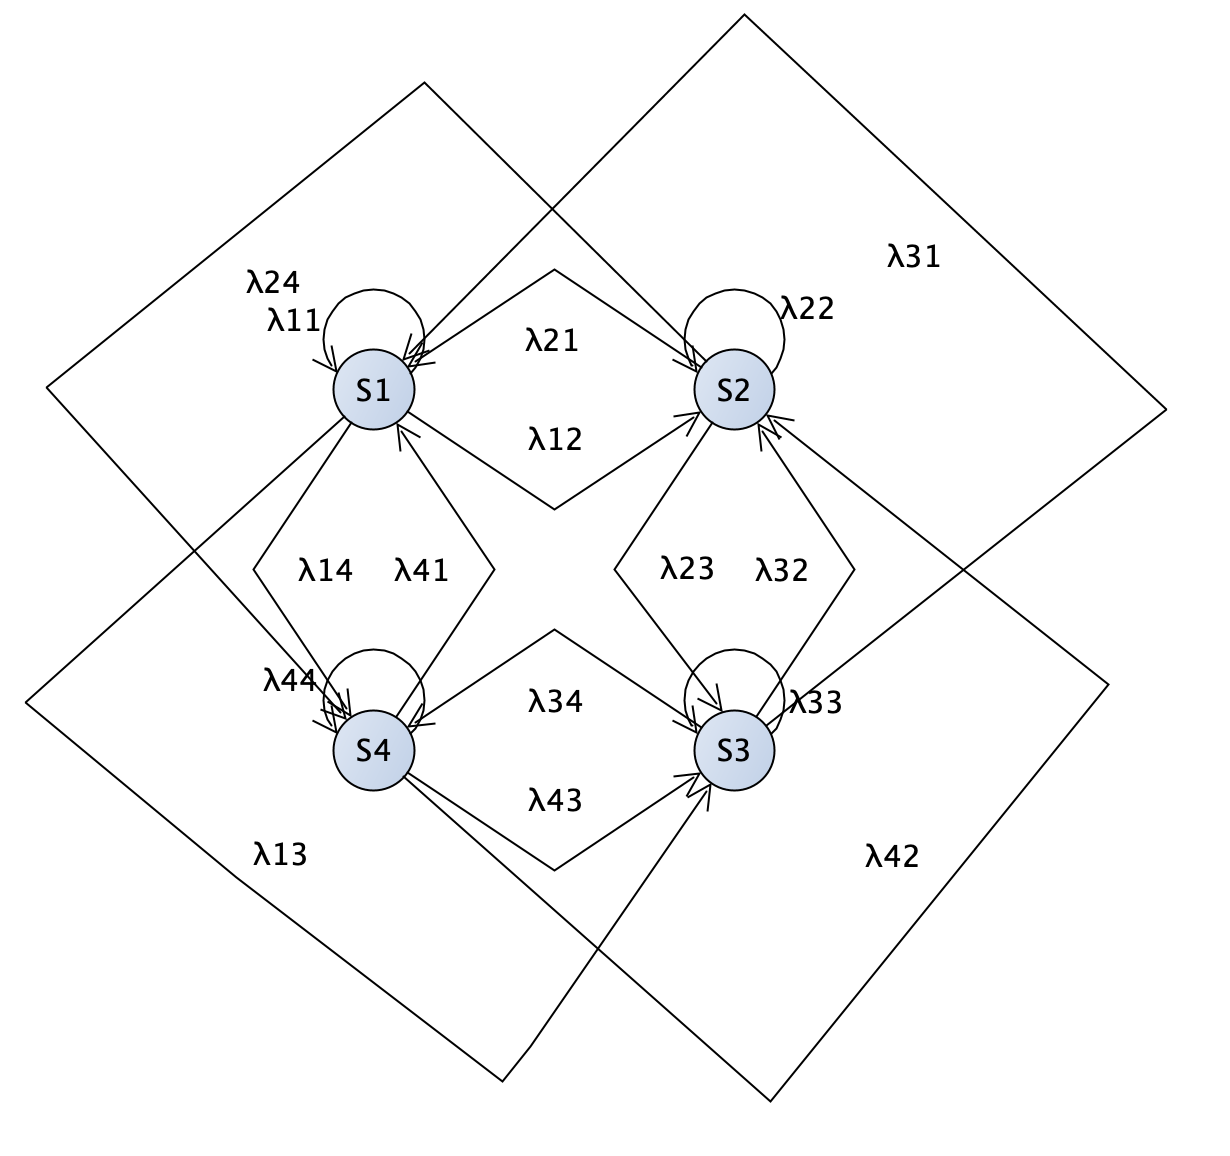
\includegraphics[scale = 0.4]{system.png}}
			\label{ris:system}
		\end{center}
		\caption{Граф марковского процесса из 4 состояний.}
	\end{figure}

	Соответственно, напишем систему уравнений для данного процесса:
	
	\begin{equation}
	\begin{cases}
		p_1'(t) = -(\lambda_{11} + \lambda_{12} + \lambda_{13} + \lambda_{14}) p_1(t) + \lambda_{11} p_1(t) + \lambda_{21} p_2(t) + \lambda_{31} p_3(t) + \lambda_{41} p_4(t)\\
		p_2'(t) = -(\lambda_{22} + \lambda_{21} + \lambda_{23} + \lambda_{24}) p_2(t) + \lambda_{22} p_2(t) + \lambda_{12} p_1(t) + \lambda_{32} p_3(t) + \lambda_{42} p_4(t)\\
		p_3'(t) = -(\lambda_{33} + \lambda_{31} + \lambda_{32} + \lambda_{34}) p_3(t) + \lambda_{33} p_3(t) + \lambda_{13} p_1(t) + \lambda_{23} p_2(t) + \lambda_{43} p_4(t)\\
		p_4'(t) = -(\lambda_{44} + \lambda_{41} + \lambda_{42} + \lambda_{43}) p_4(t) + \lambda_{44} p_4(t) + \lambda_{24} p_2(t) + \lambda_{34} p_3(t) + \lambda_{14} p_1(t)\\
	\end{cases}
	\end{equation}

	
	Вероятности состояний $p_1(t), p_2(t), p_3(t), p_4(t)$ могут быть получены решением данной системы линейных алгебраических уравнений, если по­ложить в них левые части (производные) равными нулю.
	
	Таким образом, получается (для системы S с 4 состояниями) система 4 однород­ных линейных алгебраических уравнений с 4 неизвест­ными $р_1, р_2, ..., р_4$.
	
	 
	Из этой системы можно найти неизвестные $р_1, р_2, ..., р_4$ с точностью до произвольного множителя. Чтобы найти точные значения $р_1,..., р_4$, к уравнениям добавляют нормировочное условие $p_1 + p_2+ …+ p_4 =1$, пользуясь которым можно выразить любую из ве­роятностей $p_i$ через другие (и соответственно отбросить одно из уравне­ний).

	Таким образом, система уравнений будет иметь вид:
	
	\begin{equation}
	\begin{cases}
	0 = -(\lambda_{11} + \lambda_{12} + \lambda_{13} + \lambda_{14}) p_1 + \lambda_{11} p_1 + \lambda_{21} p_2 + \lambda_{31} p_3 + \lambda_{41} p_4\\
	0 = -(\lambda_{22} + \lambda_{21} + \lambda_{23} + \lambda_{24}) p_2 + \lambda_{22} p_2 + \lambda_{12} p_1 + \lambda_{32} p_3 + \lambda_{42} p_4\\
	0 = -(\lambda_{33} + \lambda_{31} + \lambda_{32} + \lambda_{34}) p_3 + \lambda_{33} p_3 + \lambda_{13} p_1 + \lambda_{23} p_2 + \lambda_{43} p_4\\
	1 = p_1 + p_2 + p_3 + p_4\\
	\end{cases}
	\end{equation}
	
	А среднее относительное время пребывания системы в $i$-ом состоянии равняется:
	
	\begin{equation}
	\begin{cases}
	\tau_1 = \frac{(\lambda_{11} + \lambda_{12} + \lambda_{13} + \lambda_{14}) - (\lambda_{11} + \lambda_{21} + \lambda_{31} + \lambda_{41})}{p_1}\\
	\tau_2 = \frac{(\lambda_{21} + \lambda_{22} + \lambda_{23} + \lambda_{24}) - (\lambda_{12} + \lambda_{22} + \lambda_{32} + \lambda_{42})}{p_2}\\
	\tau_3 = \frac{(\lambda_{31} + \lambda_{32} + \lambda_{33} + \lambda_{34}) - (\lambda_{13} + \lambda_{23} + \lambda_{33} + \lambda_{43})}{p_3}\\
	\tau_4 = \frac{(\lambda_{41} + \lambda_{42} + \lambda_{43} + \lambda_{44}) - (\lambda_{14} + \lambda_{24} + \lambda_{34} + \lambda_{44})}{p_4}\\
	\end{cases}
	\end{equation}
	
	
	\newpage
	
	\section*{Результаты работы}
	
	Ниже приведены результаты работы программы для 3, 4 и 5 состояний.
	
	\begin{figure}[h!]
		\begin{center}
			{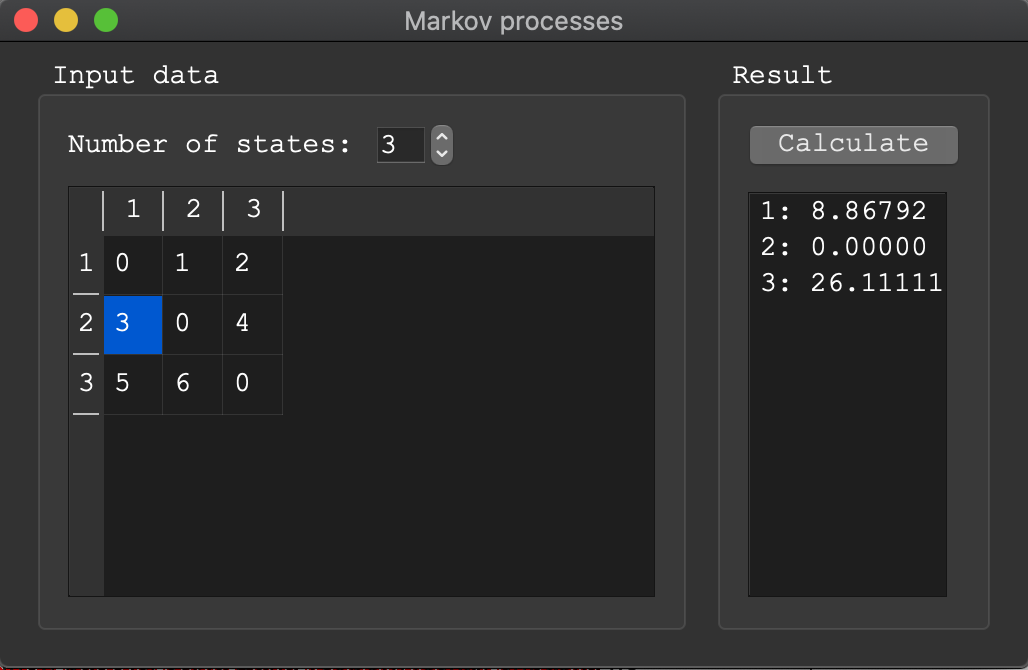
\includegraphics[scale = 0.7]{3.png}}
			\label{ris:1}
		\end{center}
		\caption{Результат работы программы при для 3 состояний.}
	\end{figure}

	\begin{figure}[h!]
		\begin{center}
			{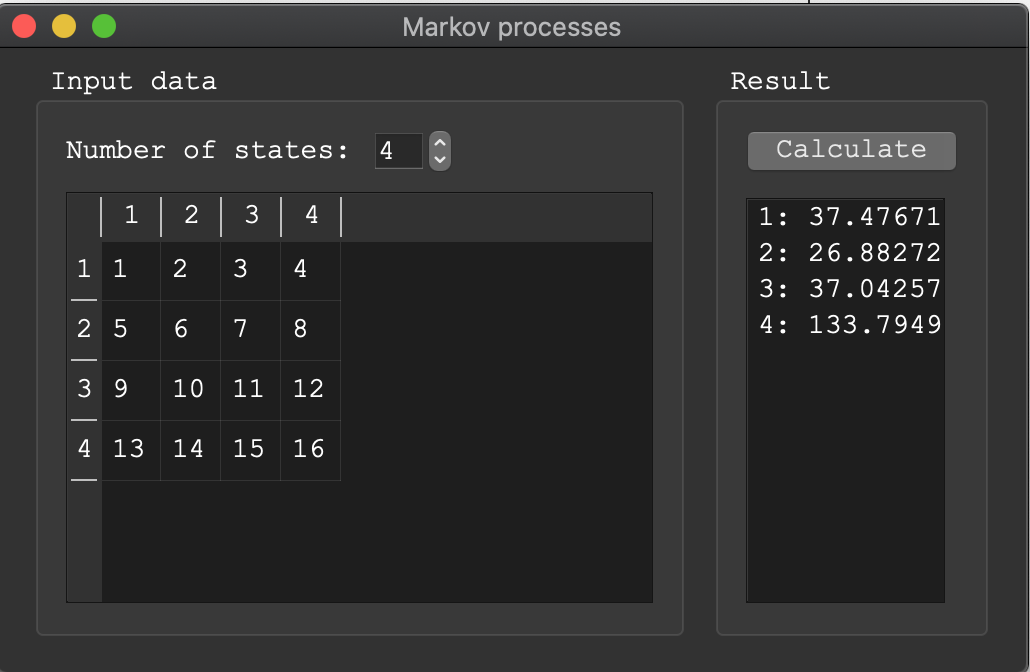
\includegraphics[scale = 0.7]{4.png}}
			\label{ris:2}
		\end{center}
		\caption{Результат работы программы при для 4 состояний.}
	\end{figure}

	\newpage

	\begin{figure}[h!]
		\begin{center}
			{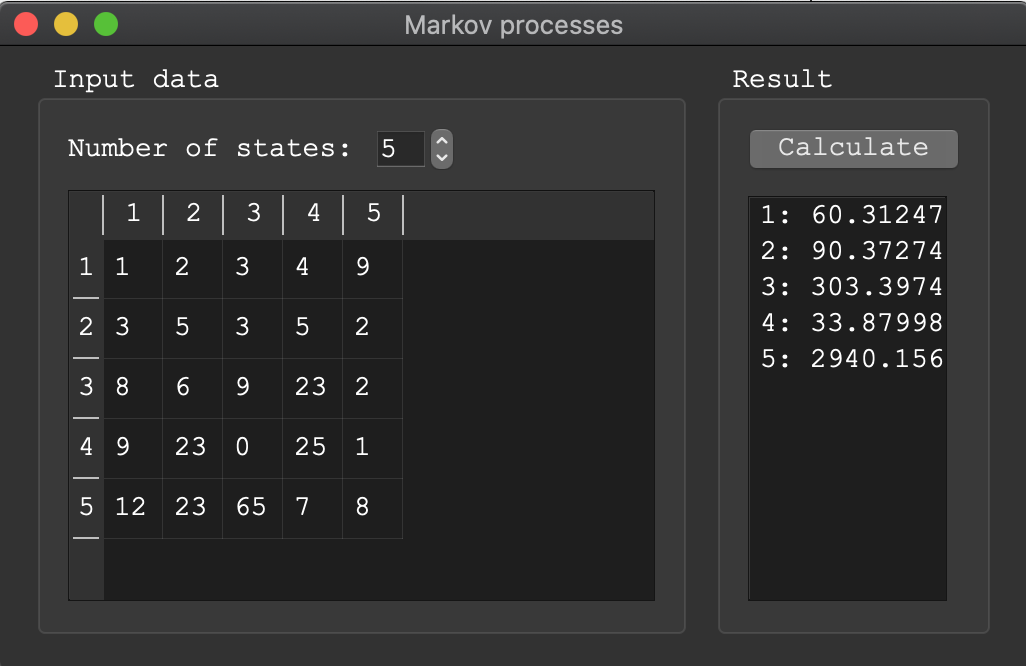
\includegraphics[scale = 0.7]{5.png}}
			\label{ris:3}
		\end{center}
		\caption{Результат работы программы при для 5 состояний.}
	\end{figure}
	
	\section*{Вывод}
	
	В результате проделанной работы была дана теоретическая справка по Марковским случайным процессам и проведена формализация задачи.
	
	Также, была разработана программа, полностью реализующая поставленную задачу. 
	
	
	
\end{document}